\chapter{Defences}
\label{ch:defences}

\Cref{ch:results} points to three defence directions:
\begin{itemize}
  \item gold at rank 0 halves the alignment gap, so retrieval precision should
    help;
  \item clustering, not volume, is what makes C1 work, so removing clusters
    should help;
  \item the aligned model's losses are visible, so its refusals might be
    monitored.
\end{itemize}
This chapter tests all three on the aligned side, which is the deployed model.
Each defence was run on the three strongest attacks plus C1, over all 1{,}000 NQ
queries, on both \pair{llama-3.1-8b} and \pair{qwen-2.5-7b}. Each defended run
is paired per query with its undefended run.

\section{Defence arms}

\begin{description}[style=nextline,leftmargin=2.8cm]
  \item[Cluster filter] Drop any candidate that has at least two
    near-duplicates (cosine $> 0.9$) in the top-50 candidate pool. The setting
    was chosen before the run.
  \item[Rerank] Reorder the top-50 pool with an MS MARCO MiniLM cross-encoder
    \cite{nogueira2019rerank}.
  \item[Cluster + rerank] Filter first, then rerank.
  \item[Prompt] No retrieval change. Remove the refusal licence from the chat
    prompt (\cref{sec:res-prompt}).
\end{description}

\begin{figure}[ht]
\centering
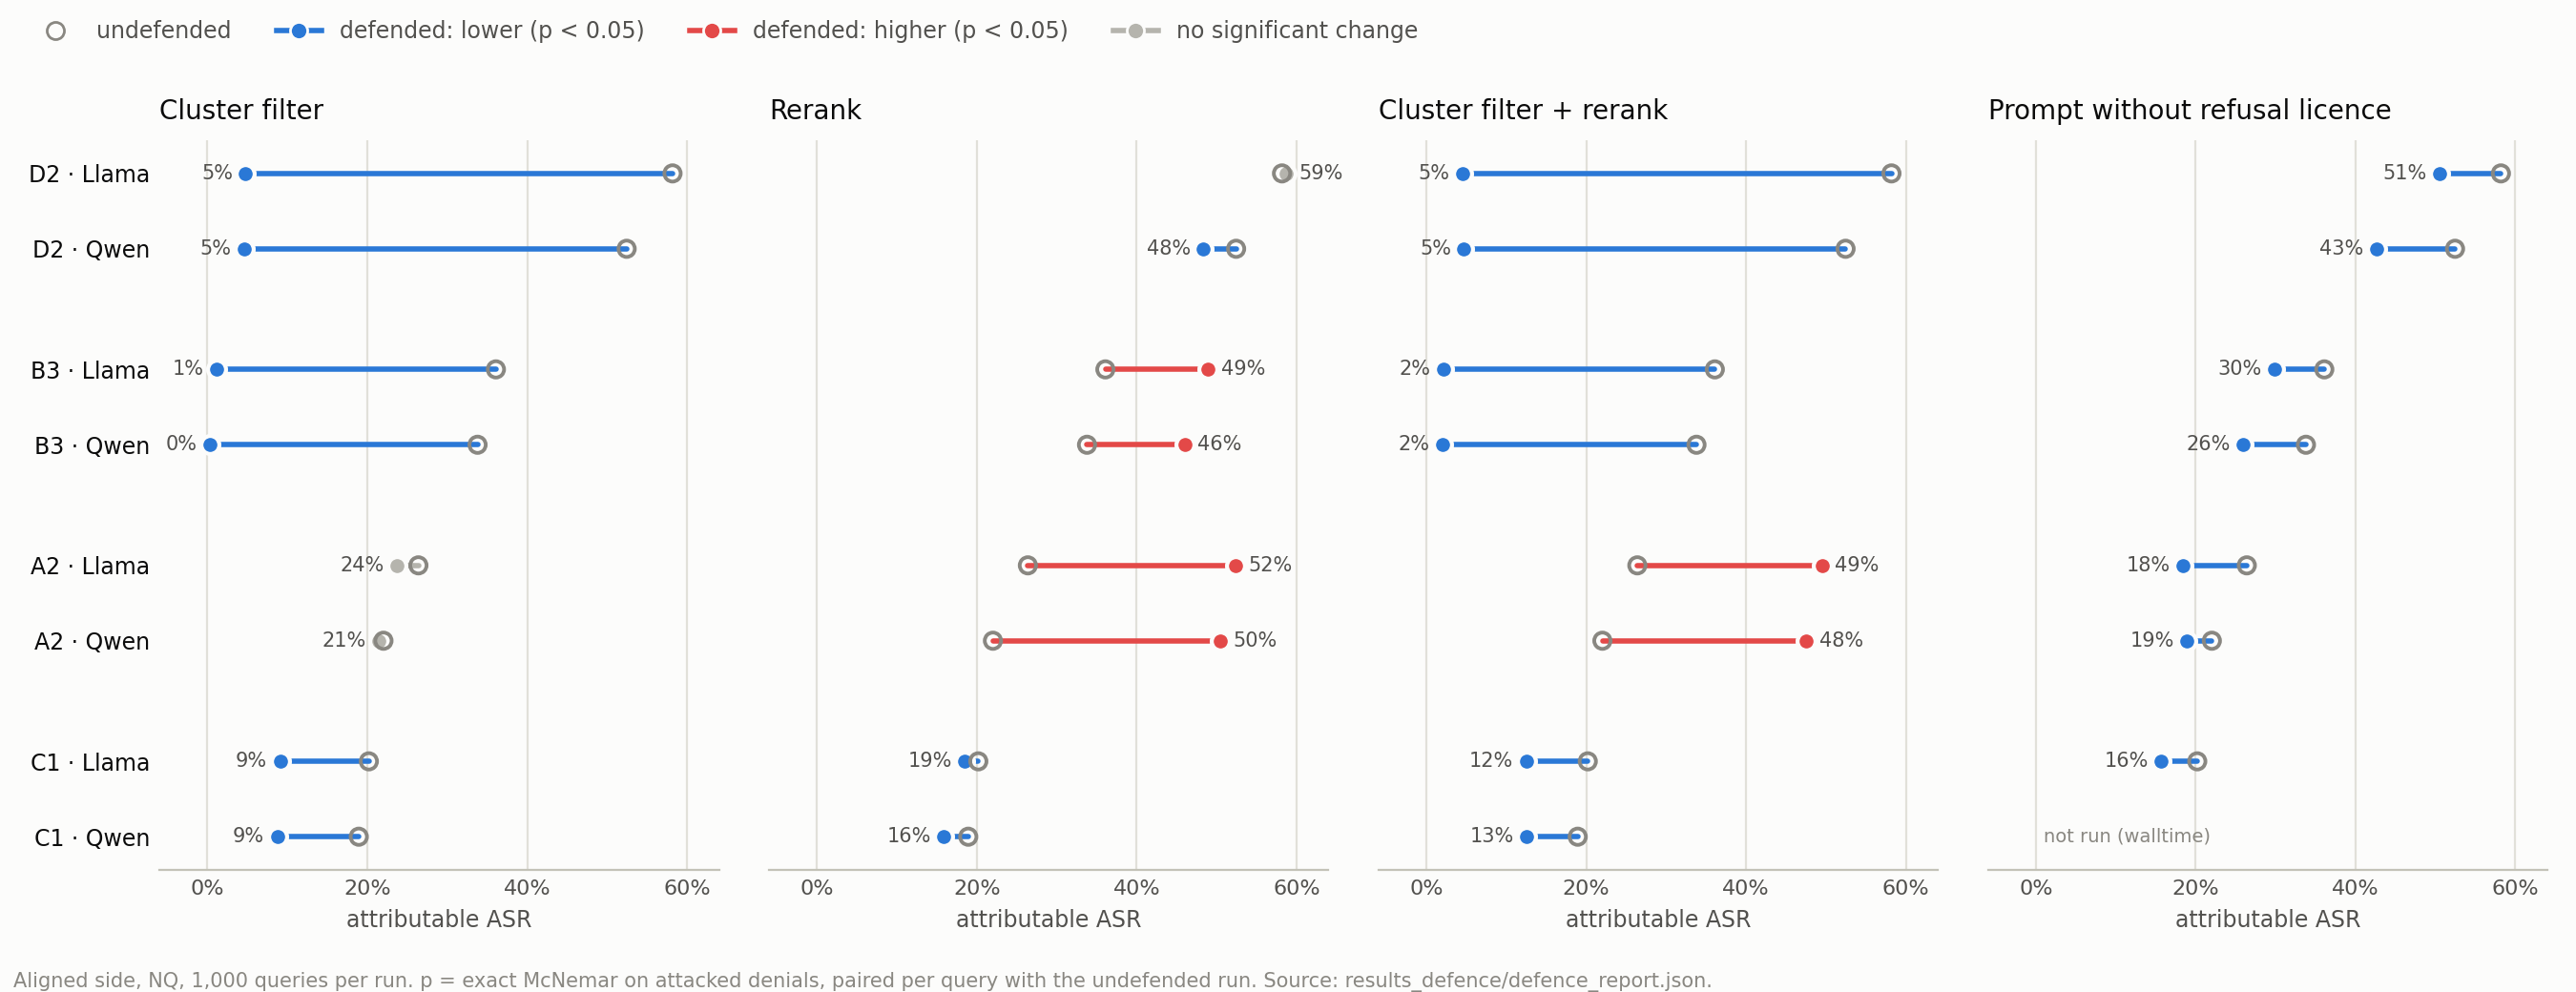
\includegraphics[width=\textwidth]{defence_asr}
\caption[Defence results]{Attributable ASR on the aligned side, undefended
(hollow ring) to defended (dot), for each attack and pair. Blue: significantly
lower (exact McNemar, $p<0.05$); red: significantly higher; grey: no
significant change.}
\label{fig:defences}
\end{figure}

\section{The cluster filter neutralises templated attacks}
\label{sec:def-cluster}

On Llama the filter cuts ASR from 58.2\% to 4.8\% on D2, from 36.1\% to 1.1\% on
B3, and from 20.2\% to 9.1\% on C1, all with $p < 10^{-17}$
(\cref{tab:defence}). Attacked denial returns to within 3.3 points of the clean
floor. Qwen replicates every cell. On clean queries nothing measurable
changes: denial 37.1\% $\to$ 37.2\% ($p=1.0$), recall@5 76.0\% $\to$ 76.1\%,
and accuracy identical. Natural NQ passages almost never have two
near-duplicates in a 50-passage pool, so the filter is close to free. This is
the intervention-level confirmation of \cref{sec:res-c1}: these attacks work
\emph{because} their passages cluster.

\begin{table}[ht]
\centering
\small
\caption[Defence ASR]{Aligned-side attributable ASR, undefended $\to$ defended,
\pair{llama-3.1-8b} (\pair{qwen-2.5-7b} in brackets).}
\label{tab:defence}
\begin{tabular}{@{}lllll@{}}
\toprule
Attack & Undefended & Cluster & Rerank & Cluster + rerank \\
\midrule
D2 & 58.2 (52.4) & \textbf{4.8} (4.6)  & 58.7 (48.3) & \textbf{4.5} (4.7) \\
B3 & 36.1 (33.8) & \textbf{1.1} (0.3)  & 48.9 (46.0) & \textbf{2.1} (2.1) \\
C1 & 20.2 (18.9) & \textbf{9.1} (8.7)  & 18.5 (15.8) & 12.5 (12.5) \\
A2 & 26.4 (22.0) & 23.7 (21.4)          & 52.4 (50.4) & 49.5 (47.5) \\
\bottomrule
\end{tabular}
\end{table}

\paragraph{A2 evades it.} Contradiction flooding writes its passages as distinct
claim pairs rather than templated copies, so few of them clear the similarity
threshold. ASR falls by only 2.7 points, which is not significant. The filter is
a defence against \emph{templated} poisoning, not against poisoning in
general.

\paragraph{The setting is not cherry-picked.} Because the filter acts only on
retrieval, 27 settings could be replayed offline on recorded candidate pools.
With two neighbours, any threshold from 0.85 to 0.92 gives the same protection
at no recall cost, so 0.9 sits on a plateau. Requiring three neighbours allows
a looser threshold of 0.83. That removes two-thirds of A2's passages from the
top-5 (2.06 $\to$ 0.67) with clean recall unchanged. The setting was selected
on queries 0--499 and confirmed on 500--999. \todo{Generation run at
$\tau=0.83$, $\geq$3 neighbours is on Katana; until it lands this is a
retrieval-only result.}

\section{Reranking amplifies the attacks}
\label{sec:def-rerank}

On clean queries the reranker is the best retrieval arm. Gold at rank 0 rises
from 47.2\% to 59.8\%, and clean refusals fall by 3.5 points, which is
\cref{sec:res-mechanism}'s rank-0 effect shown by intervention. Under attack,
however, it pulls \emph{more} adversarial passages into the top-5 (A2: 2.05
$\to$ 4.41). A2's ASR doubles to 52.4\%, and B3's rises to 48.9\%. The attack
passages restate the query, and a relevance model rewards exactly that.
\textbf{A standard RAG hardening step makes these denial attacks stronger.}

Order matters when the two are combined. Filtering first keeps the filter's
protection on D2, B3 and C1 \emph{and} the reranker's clean gains (recall 84\%,
accuracy 50\%), which makes it the best arm overall. The exception is A2: its
passages survive the filter, and the reranker then promotes them.

\section{The prompt is not a defence}

Removing the refusal licence lowers denial everywhere, clean (37\% $\to$ 24\%)
as much as attacked. It leaves the retrieved adversarial passages unchanged,
and residual ASR stays high (D2 50.5\%). It moves the refusal floor rather than
defending against the attack.

\section{Can refusals be monitored?}
\label{sec:def-monitor}

\Cref{tab:failmode} suggested that the aligned model's refusals are a signal an
operator can act on. A single refusal is not. Attack-induced refusals read like
ordinary ones, and the classifier puts both in the same class. A monitor must
therefore watch the refusal \emph{rate}. Calibrated on queries 0--499, a
one-sided binomial alarm at $\alpha = 0.01$ was simulated on the held-out half,
with a fraction $f$ of each window attacked.

\begin{table}[ht]
\centering
\small
\caption[Refusal-rate monitor]{Smallest window (queries) that detects the
attack with $\geq$90\% power. ---: not detected within 500.}
\label{tab:monitor}
\begin{tabular}{@{}lllll@{}}
\toprule
Aligned side & D2 & B3 & A2 & C1 \\
\midrule
\pair{llama-3.1-8b}, $f=1$ & 50  & 150 & 300 & --- \\
\pair{qwen-2.5-7b}, $f=1$  & 50  & 150 & 300 & 500 \\
\pair{mistral-7b}, $f=1$   & 100 & 100 & 200 & n/a \\
any pair, $f \leq 0.25$    & --- & --- & --- & --- \\
\bottomrule
\end{tabular}
\end{table}

The asymmetry is real: no base model emits a usable signal. But on the aligned
side the 31--41\% clean floor is noise the attack has to rise above. Detection
needs tens to hundreds of queries, all of them attacked, and an attacker who
poisons a quarter of traffic is never caught. The floor that makes the aligned
model look vulnerable also hides the attack from the monitor.

\section{Limitations of the defence study}
\begin{itemize}
  \item Aligned side only, on two pairs and NQ only.
    \todo{Base-side cluster-filter runs are on Katana: does the alignment gap
    close under the filter?}
  \item The attacker is non-adaptive. A2 already shows how an adaptive
    attacker evades the filter.
  \item Each arm has its own clean-answerable denominator, so ASR is not
    paired across arms. Attacked denial and accuracy are paired.
\end{itemize}
